\documentclass[spanish, c]{beamer}

\usepackage[utf8]{inputenc}
\usepackage[spanish, mexico]{babel}
\usepackage{amsmath}
\usepackage{mathtools}
\usepackage{hyperref}
\usepackage{xcolor}
\usepackage{color}
\usepackage{ragged2e}
\usepackage{mathrsfs}
\usepackage{csquotes}
\usepackage{listings}
\usepackage[scaled]{beramono}
\usepackage[T1]{fontenc}
\usepackage{matlab-prettifier}
\usepackage{graphicx}
\usepackage{booktabs}
\usepackage{tikz}
\usepackage{venndiagram}
\usepackage{semantic}

\renewcommand{\indent}{\hspace*{2em}}

% \usetikzlibrary{fit, shapes, arrows}

% \usepackage{courier}
% \usepackage{subfigure}
% \usepackage{enumerate}
% \usepackage{algorithmic}
% \usepackage{algorithm}

% \usepackage{listings}
% \usepackage{lstlinebgrd}

\usetheme{Boadilla}
\usefonttheme[onlymath]{serif}

\newcommand{\matlab}[1]{\lstinline[style=Matlab-editor]!#1!}
\newcommand\blfootnote[1]{%
\begingroup
\renewcommand\thefootnote{}\footnote{#1}%
\addtocounter{footnote}{-1}%
\endgroup
}

\lstset
{
    language = Matlab,
    style = Matlab-editor,
    basicstyle = \mlttfamily\scriptsize,
    escapechar = `,
    numbers = left,
    frame = tb,
}

\lstdefinestyle{output}
{
    language = {},
    basicstyle = \mlttfamily\scriptsize,
    escapechar = `,
    numbers = none,
    showtabs = false,
   	showstringspaces = false,
}

% Sets the templates
\definecolor{navyblue}{RGB}{0, 0, 128}
\definecolor{crimson}{RGB}{128, 16, 0}

\setbeamertemplate{navigation symbols}{}
\setbeamertemplate{headline}{}
\setbeamertemplate{title page}[default][colsep=-4bp,rounded=true]
\setbeamertemplate{footline}[frame number]
\setbeamertemplate{bibliography item}[text]
\setbeamertemplate{theorems}[numbered]

\setbeamercolor{title}{fg=navyblue, bg=white}
\setbeamercolor{frametitle}{fg=navyblue, bg=white}
\setbeamercolor{structure}{fg=navyblue}
\setbeamercolor{button}{fg=white,bg=navyblue}

\setbeamercovered{transparent}

\title{Grafos II: Aplicaciones y características}
\subtitle{Matemáticas Discretas \\ (TC1003)}
\author{
    \texorpdfstring{
        \begin{center}
            M.C. Xavier Sánchez Díaz \\
            \href{mailto:sax@tec.mx}{\texttt{sax@tec.mx}}
        \end{center}
    }
    {M.C. Xavier Sánchez Díaz}
}

\institute[Tecnológico de Monterrey]{\includegraphics[scale=0.5]{../img/logo}}
\date{}

\begin{document}

\setlength{\rightskip}{0pt}

\begin{frame}[plain]
    \titlepage        
\end{frame}

\begin{frame}{Outline}
    \tableofcontents
\end{frame}

\section{Grafos especiales}

\begin{frame}{Grafos bipartito}{Grafos especiales}
    Un grafo $G = (V,E)$ se dice que es \alert{bipartito} si $V = V_1 \cup V_2$ tal que no existen ejes que \textbf{interconecten} $V_1$ o $V_2$
    \begin{center}
        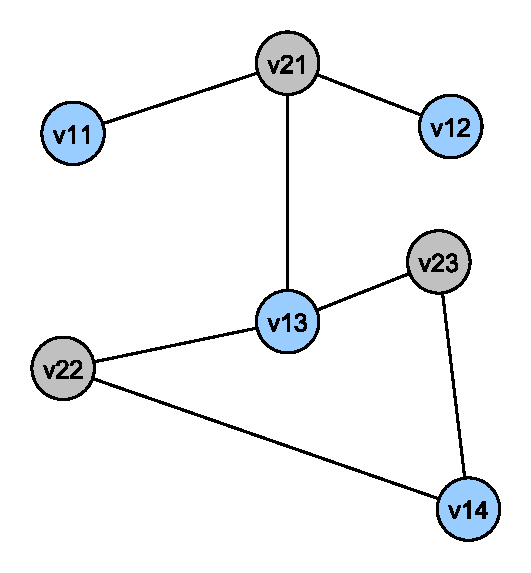
\includegraphics[width=0.4\textwidth]{bipartite.pdf}
    \end{center}
    En otras palabras, si todos los ejes que salen de $v_i \in V_1$ llegan a $v_j \in V_2$ y viceversa.
\end{frame}

\begin{frame}{Grafos $K$}{Grafos Especiales}
    Un grafo \textbf{completo} $\alert{K_n}$ es un grafo con $n$ vértices y con todos los ejes posibles, que también es \alert{$n-1$-regular}.

    \begin{center}
        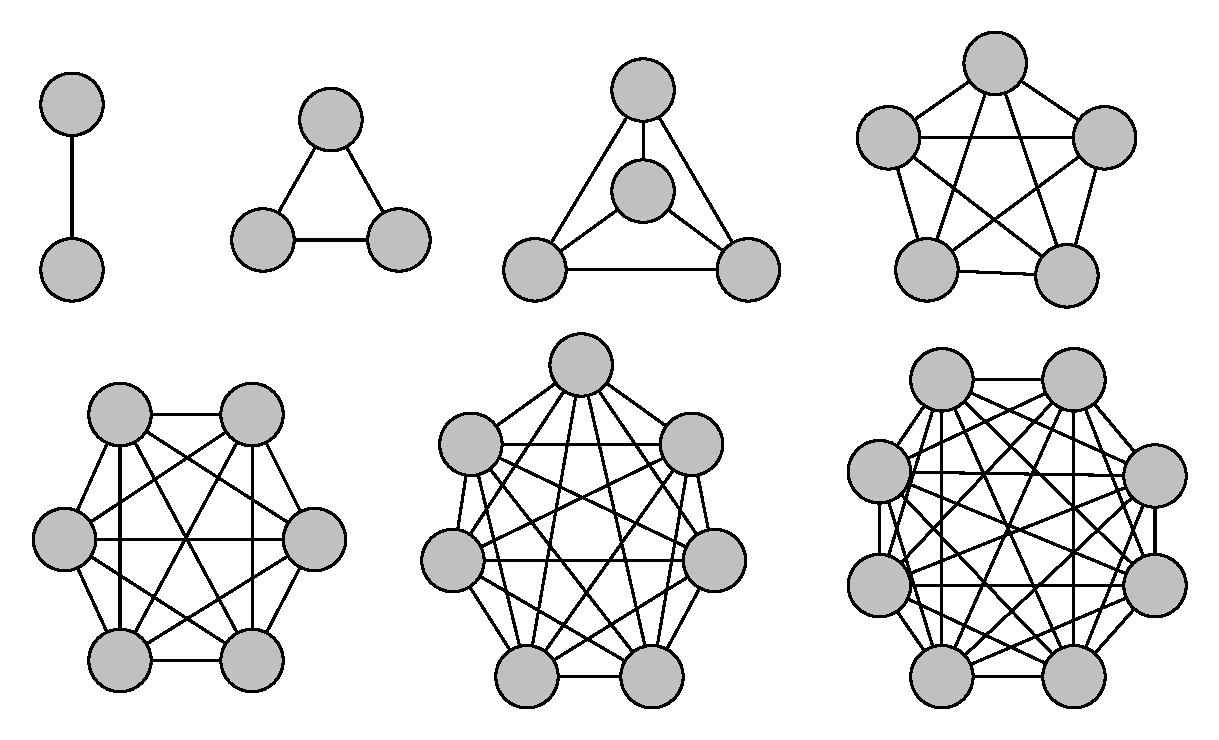
\includegraphics[width=0.8\textwidth]{kgraph.pdf}
    \end{center}
\end{frame}

\section{Representaciones con matrices}

\begin{frame}{Matriz de adyacencia}{Representaciones con matrices}
    Una matriz de \alert{adyacencia} $n \times m$ puede representar en su celda $A_{i,j}$ si existe un eje entre el vértice $i$ y el vértice $j$:

    \begin{columns}
        \begin{column}{0.5\textwidth}
            $$A = \begin{bmatrix}%
                0 & 0 & 0 & 1 & 0 \\
                0 & 0 & 1 & 0 & 1 \\
                0 & 1 & 0 & 1 & 1 \\
                1 & 0 & 1 & 0 & 1 \\
                0 & 1 & 1 & 1 & 0
            \end{bmatrix}$$
        \end{column}
        \begin{column}{0.5\textwidth}
            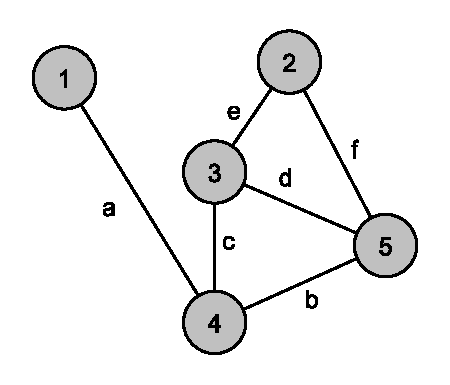
\includegraphics[width=\textwidth]{adj-inc.pdf}
        \end{column}
    \end{columns}
\end{frame}

\begin{frame}{Matriz de incidencia}{Representaciones con matrices}
    Una matriz de \alert{incidencia} $n \times m$ puede representar en sus celdas $T_{i,k} = T_{j,k}$ si el eje $k$ tiene como extremos a los vértices $i$ y $j$:

    \begin{columns}
        \begin{column}{0.5\textwidth}
            $$A = \begin{bmatrix}%
                1 & 0 & 0 & 0 & 0 & 0 \\
                0 & 0 & 0 & 0 & 1 & 1 \\
                0 & 0 & 1 & 1 & 1 & 0 \\
                1 & 1 & 1 & 0 & 0 & 0 \\
                0 & 1 & 0 & 1 & 0 & 1
            \end{bmatrix}$$
        \end{column}
        \begin{column}{0.5\textwidth}
            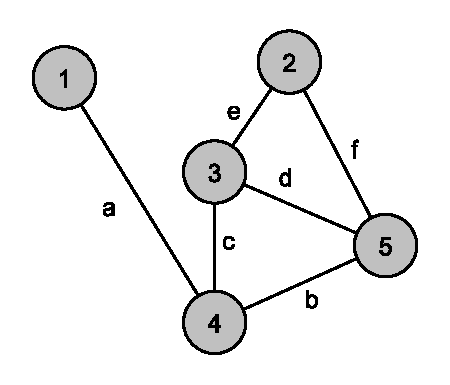
\includegraphics[width=\textwidth]{adj-inc.pdf}
        \end{column}
    \end{columns}
\end{frame}

\section{Operaciones con grafos}

\begin{frame}{Componentes fuertemente conectados}{Operaciones con grafos}
En un \textbf{grafo direccionado}, dos vértices $u$ y $v$ están \alert{fuertemente conectados} si existe una \textbf{caminata} de $u$ a $v$ y de $v$ a $u$.

\bigskip

Podemos agrupar los \textbf{componentes fuertemente conectados} para reducir el grafo.

\begin{center}
    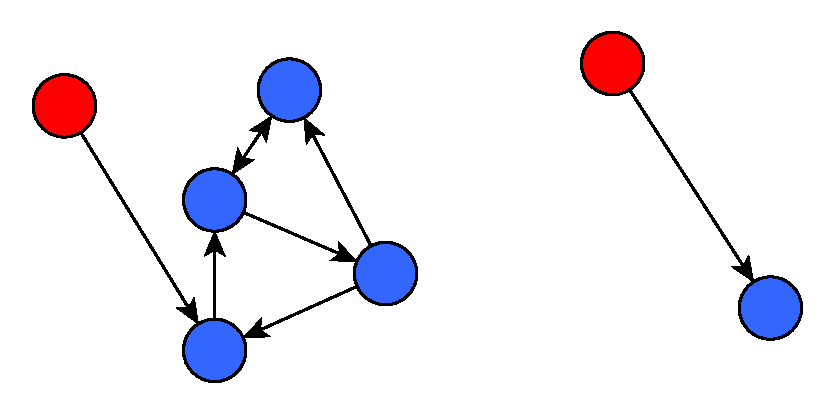
\includegraphics[width=0.7\textwidth]{stronglyconnected.pdf}
\end{center}
\end{frame}

\begin{frame}{Búsqueda}{Operaciones con grafos}
    Podemos hacer una \alert{búsqueda} en un grafo para marcar los vértices encontrados y generar una secuencia. Empezando en el 1, podemos buscar por \alert{profundidad}:
    \begin{center}
        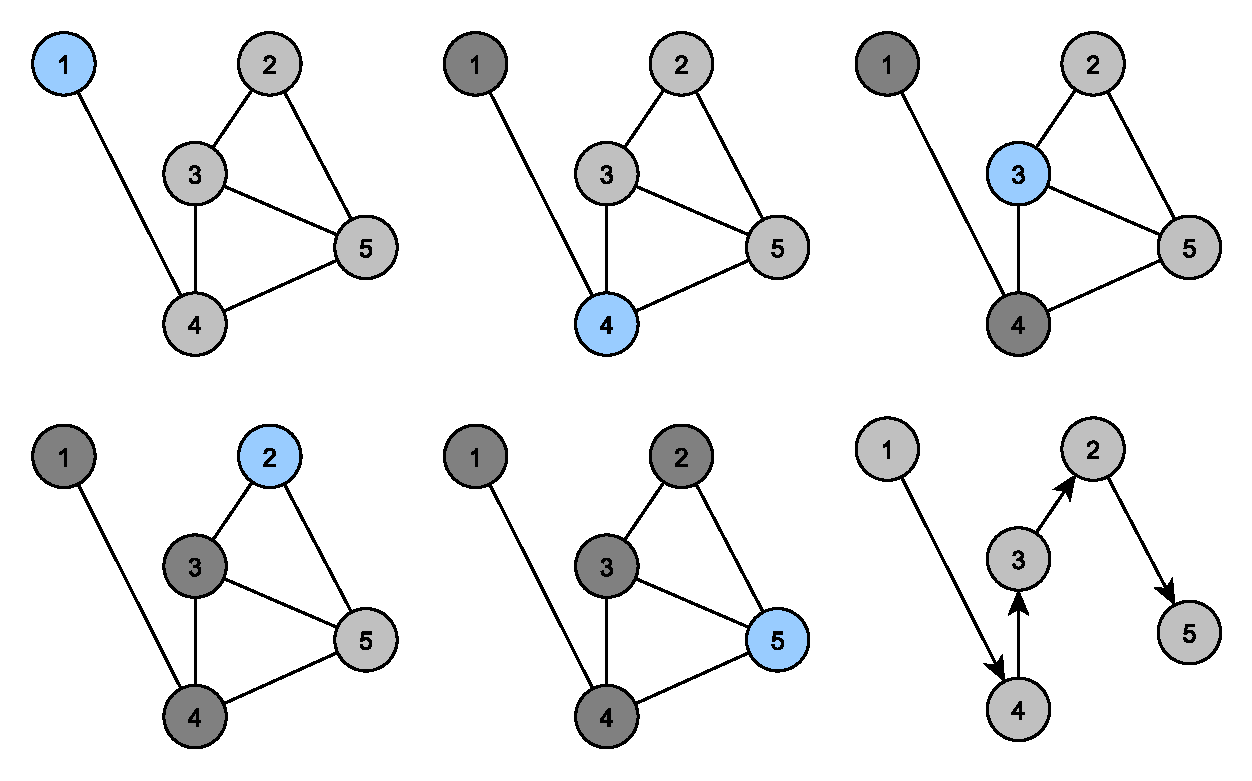
\includegraphics[width=0.85\textwidth]{dfs.pdf}
    \end{center}
\end{frame}

\begin{frame}{Búsqueda}{Operaciones con grafos}
    O bien podemos buscar por \alert{anchura}:
    \begin{center}
        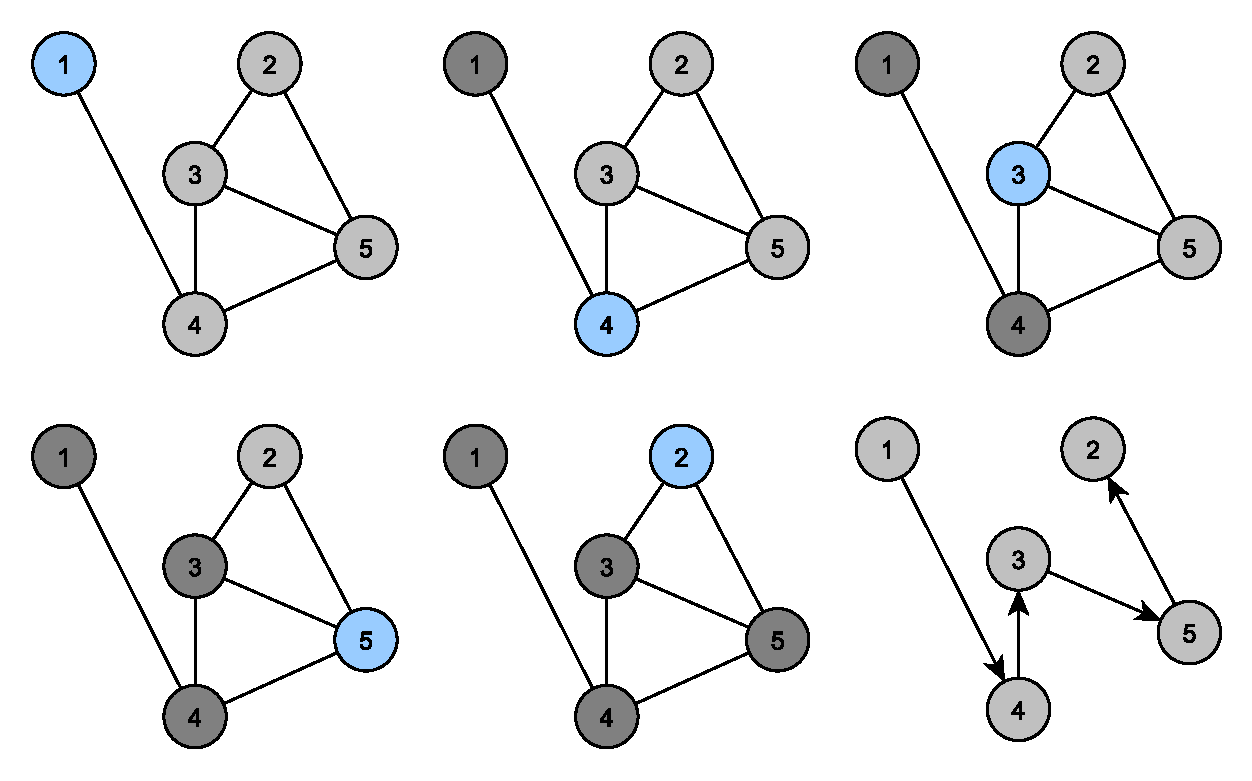
\includegraphics[width=0.85\textwidth]{bfs.pdf}
    \end{center}
\end{frame}

\section{Árboles}

\begin{frame}{Árboles}
    El \textbf{orden} de los nodos de un grafo dan pie a una jerarquía, lo cual es usualmente representado con un grafo acíclico que conocemos como \alert{árbol}.
    \begin{center}
        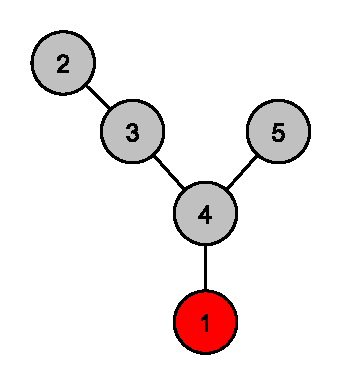
\includegraphics[width=0.3\textwidth]{tree.pdf}
    \end{center}
    Un \textbf{árbol} es una estructura de datos \textit{ordenada}, donde el nodo \alert{raíz} es \alert{padre} de algunos otros nodos \alert{hijos}. Los nodos \textit{finales}, los que no tienen descendencia, se les conoce como nodos \alert{hoja}, y suelen representarse con la raíz hasta arriba\dots
\end{frame}

\begin{frame}{Definición Recursiva}{Árboles}
\dots así. Un árbol puede ser definido de manera \textbf{recursiva}, considerando que tiene la misma estructura replicada múltiples veces.
\begin{center}
    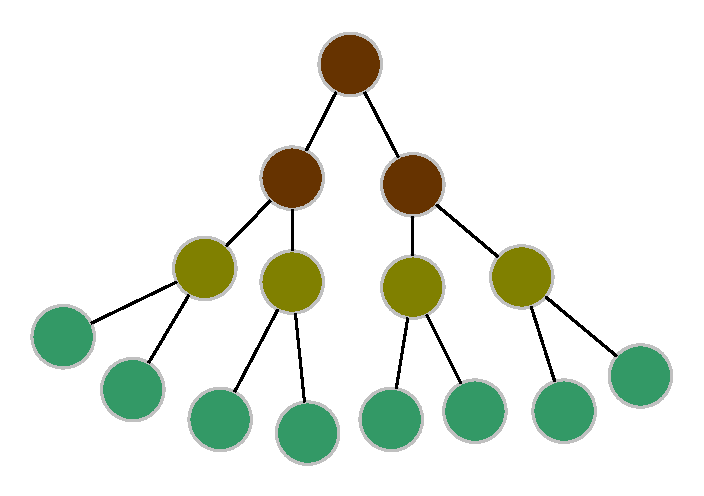
\includegraphics[width=0.6\textwidth]{binarytree.pdf}
\end{center}
En un \alert{árbol binario}, cada vértice padre tiene dos nodos hijos---uno izquierdo y uno derecho---que a su vez tienen cada uno dos nodos hijos\dots
\end{frame}

\section{Aplicaciones de alta complejidad}

\begin{frame}[t]{Aplicaciones de alta complejidad}
    \vspace{-2ex}
    Como ya vimos, muchas situaciones problema pueden ser representadas con grafos. Sin embargo, existen algunos problemas \textit{clásicos} que suelen estudiarse (y que no son parte del índice analítico pero es bueno que conozcan).
    \bigskip
    \begin{columns}
        \begin{column}{0.5\textwidth}
            \begin{itemize}
                \slshape
                \item Max-flow
                \item Min-cut
                \item Max-flow Min-cut
                \item Minimum spanning tree
                \item Eulerian tour
                \item Chinese Postman
            \end{itemize}
        \end{column}
        \begin{column}{0.5\textwidth}
            \begin{itemize}
                \slshape
                \item Hamiltonian cycle
                \item Traveling Salesman
                \item Graph-coloring
                \item Constraint Satisfaction
                \item K-satisfiability
            \end{itemize}
        \end{column}
    \end{columns}

    \bigskip

    Todos los de la derecha son de la clase $\mathcal{NP}$\textit{-complete}\footnote{Véase \url{https://en.wikipedia.org/wiki/List\_of\_NP-complete\_problems}}. Si alguien encuentra cómo resolverlos de manera óptima, por favor envíeme un correo.

\end{frame}

\section{CSPs}

\begin{frame}{Satisfacción de Restricciones}{CSPs}

    Un problema de \alert{satisfacción de restricciones} se define como una tripleta $P = (X, D, C)$ donde

    \begin{itemize}
        \item $X$ es un conjunto de variables,
        \item $D$ es un conjunto de dominios de dichas variables (los valores que pueden tomar), y
        \item $C$ es un conjunto de restricciones
    \end{itemize}

    en donde la solución es verdadera o falsa dependiendo de la existencia de un mapeo $f \colon X_i \to D_i, \forall i \in X, i \in D$ en el que ninguna restricción $c \in C$ sea violada.
    
\end{frame}
% \section*{Referencias}

% \begin{frame}[t]{Referencias}
    % \nocite{bibID01}
    % \nocite{bibID02}

    % \bibliographystyle{IEEE}
    % \bibliography{biblio}
% \end{frame}

\end{document}